% Created by tikzDevice version 0.12.3.1 on 2022-09-02 16:27:19
% !TEX encoding = UTF-8 Unicode
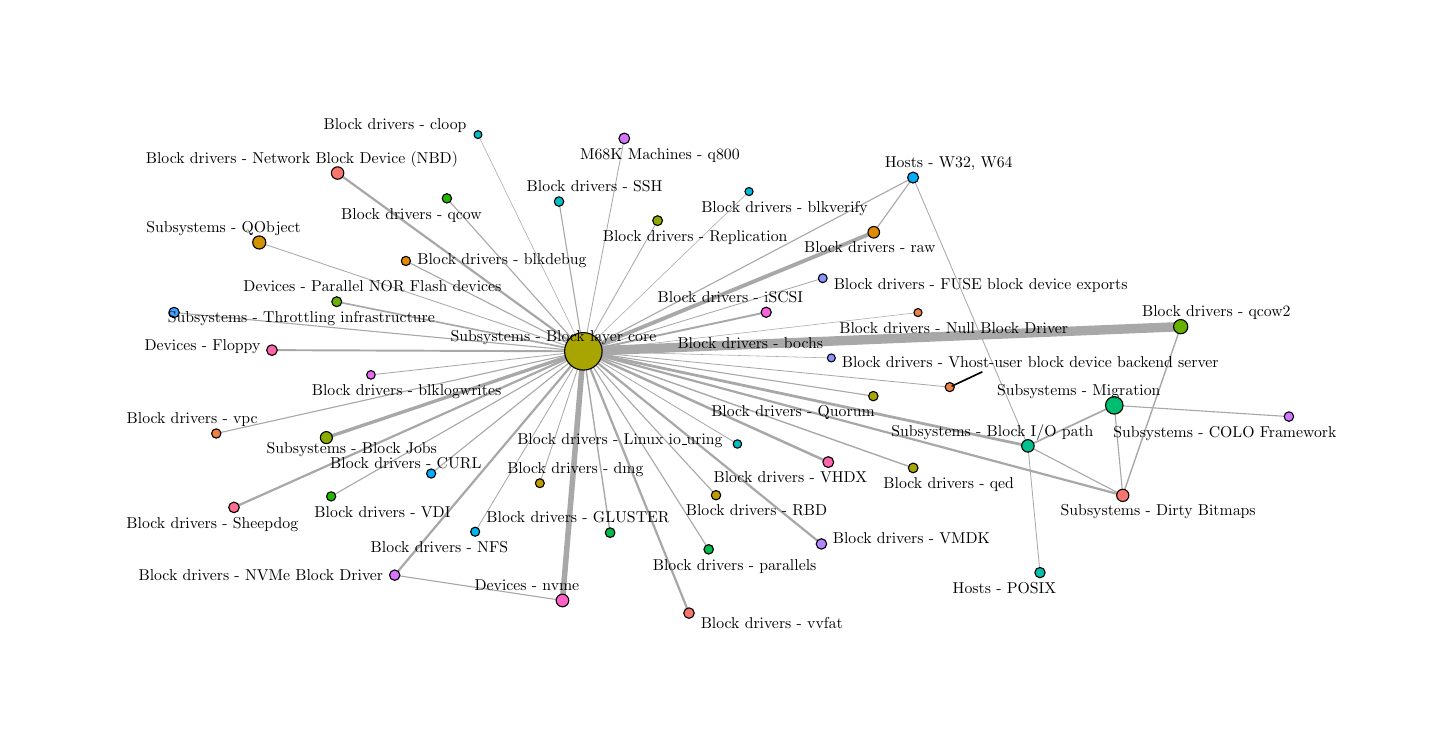
\begin{tikzpicture}[x=1pt,y=1pt]
\definecolor{fillColor}{RGB}{255,255,255}
\path[use as bounding box,fill=fillColor,fill opacity=0.00] (0,0) rectangle (505.89,252.94);
\begin{scope}
\path[clip] (  0.00,  0.00) rectangle (505.89,252.94);
\definecolor{fillColor}{RGB}{255,255,255}

\path[fill=fillColor] (  0.00,  0.00) rectangle (505.89,252.94);
\end{scope}
\begin{scope}
\path[clip] ( 32.75, 32.75) rectangle (475.89,222.94);
\definecolor{drawColor}{gray}{0.66}

\path[draw=drawColor,line width= 0.4pt,line join=round] (145.80, 91.83) -- (200.80,135.98);

\path[draw=drawColor,line width= 0.3pt,line join=round] (287.30,162.39) -- (200.80,135.98);

\path[draw=drawColor,line width= 0.5pt,line join=round] (210.47, 70.46) -- (200.80,135.98);

\path[draw=drawColor,line width= 0.3pt,line join=round] (256.47,102.50) -- (200.80,135.98);

\path[draw=drawColor,line width= 0.3pt,line join=round] (161.70, 70.80) -- (200.80,135.98);

\path[draw=drawColor,line width= 0.4pt,line join=round] (132.63, 55.11) -- (193.24, 45.95);

\path[draw=drawColor,line width= 0.8pt,line join=round] (132.63, 55.11) -- (200.80,135.98);

\path[draw=drawColor,line width= 0.8pt,line join=round] (111.99,200.41) -- (200.80,135.98);

\path[draw=drawColor,line width= 0.2pt,line join=round] (321.71,149.99) -- (200.80,135.98);

\path[draw=drawColor,line width= 0.4pt,line join=round] (305.58,119.80) -- (200.80,135.98);

\path[draw=drawColor,line width= 0.4pt,line join=round] (248.73, 83.99) -- (200.80,135.98);

\path[draw=drawColor,line width= 0.3pt,line join=round] (227.62,183.21) -- (200.80,135.98);

\path[draw=drawColor,line width= 0.4pt,line join=round] (192.00,190.11) -- (200.80,135.98);

\path[draw=drawColor,line width= 0.8pt,line join=round] ( 74.55, 79.59) -- (200.80,135.98);

\path[draw=drawColor,line width= 0.4pt,line join=round] (109.66, 83.57) -- (200.80,135.98);

\path[draw=drawColor,line width= 0.9pt,line join=round] (289.29, 95.96) -- (200.80,135.98);

\path[draw=drawColor,line width= 0.8pt,line join=round] (286.82, 66.39) -- (200.80,135.98);

\path[draw=drawColor,line width= 0.3pt,line join=round] (333.18,123.06) -- (200.80,135.98);

\path[draw=drawColor,line width= 0.4pt,line join=round] (136.67,168.64) -- (200.80,135.98);

\path[draw=drawColor,line width= 0.3pt,line join=round] (124.03,127.48) -- (200.80,135.98);

\path[draw=drawColor,line width= 0.2pt,line join=round] (260.66,193.72) -- (200.80,135.98);

\path[draw=drawColor,line width= 0.2pt,line join=round] (290.41,133.59) -- (200.80,135.98);

\path[draw=drawColor,line width= 0.2pt,line join=round] (162.72,214.30) -- (200.80,135.98);

\path[draw=drawColor,line width= 0.3pt,line join=round] (185.07, 88.33) -- (200.80,135.98);

\path[draw=drawColor,line width= 0.7pt,line join=round] (266.86,150.10) -- (200.80,135.98);

\path[draw=drawColor,line width= 0.4pt,line join=round] (246.08, 64.43) -- (200.80,135.98);

\path[draw=drawColor,line width= 0.4pt,line join=round] (151.48,191.26) -- (200.80,135.98);

\path[draw=drawColor,line width= 3.4pt,line join=round] (416.64,144.90) -- (200.80,135.98);

\path[draw=drawColor,line width= 0.5pt,line join=round] (416.64,144.90) -- (395.71, 83.94);

\path[draw=drawColor,line width= 0.5pt,line join=round] (319.98, 93.85) -- (200.80,135.98);

\path[draw=drawColor,line width= 0.4pt,line join=round] (305.73,179.00) -- (319.94,198.78);

\path[draw=drawColor,line width= 1.4pt,line join=round] (305.73,179.00) -- (200.80,135.98);

\path[draw=drawColor,line width= 0.4pt,line join=round] ( 68.14,106.30) -- (200.80,135.98);

\path[draw=drawColor,line width= 0.8pt,line join=round] (238.97, 41.40) -- (200.80,135.98);

\path[draw=drawColor,line width= 0.7pt,line join=round] ( 88.27,136.42) -- (200.80,135.98);

\path[draw=drawColor,line width= 0.6pt,line join=round] (111.68,153.91) -- (200.80,135.98);

\path[draw=drawColor,line width= 2.0pt,line join=round] (193.24, 45.95) -- (200.80,135.98);

\path[draw=drawColor,line width= 0.3pt,line join=round] (365.80, 56.03) -- (361.43,101.82);

\path[draw=drawColor,line width= 0.3pt,line join=round] (319.94,198.78) -- (361.43,101.82);

\path[draw=drawColor,line width= 0.4pt,line join=round] (319.94,198.78) -- (200.80,135.98);

\path[draw=drawColor,line width= 0.3pt,line join=round] (215.59,212.91) -- (200.80,135.98);

\path[draw=drawColor,line width= 1.0pt,line join=round] (361.43,101.82) -- (200.80,135.98);

\path[draw=drawColor,line width= 0.4pt,line join=round] (361.43,101.82) -- (395.71, 83.94);

\path[draw=drawColor,line width= 0.6pt,line join=round] (361.43,101.82) -- (392.64,116.46);

\path[draw=drawColor,line width= 1.2pt,line join=round] (107.93,104.81) -- (200.80,135.98);

\path[draw=drawColor,line width= 0.8pt,line join=round] (200.80,135.98) -- (395.71, 83.94);

\path[draw=drawColor,line width= 0.3pt,line join=round] (200.80,135.98) -- ( 83.68,175.32);

\path[draw=drawColor,line width= 0.4pt,line join=round] (200.80,135.98) -- ( 52.89,150.01);

\path[draw=drawColor,line width= 0.4pt,line join=round] (455.75,112.41) -- (392.64,116.46);

\path[draw=drawColor,line width= 0.4pt,line join=round] (395.71, 83.94) -- (392.64,116.46);
\definecolor{drawColor}{RGB}{0,0,0}
\definecolor{fillColor}{RGB}{0,172,252}

\path[draw=drawColor,line width= 0.4pt,line join=round,line cap=round,fill=fillColor] (145.80, 91.83) circle (  1.66);
\definecolor{fillColor}{RGB}{139,147,255}

\path[draw=drawColor,line width= 0.4pt,line join=round,line cap=round,fill=fillColor] (287.30,162.39) circle (  1.60);
\definecolor{fillColor}{RGB}{0,187,73}

\path[draw=drawColor,line width= 0.4pt,line join=round,line cap=round,fill=fillColor] (210.47, 70.46) circle (  1.75);
\definecolor{fillColor}{RGB}{0,191,196}

\path[draw=drawColor,line width= 0.4pt,line join=round,line cap=round,fill=fillColor] (256.47,102.50) circle (  1.53);
\definecolor{fillColor}{RGB}{0,181,237}

\path[draw=drawColor,line width= 0.4pt,line join=round,line cap=round,fill=fillColor] (161.70, 70.80) circle (  1.64);
\definecolor{fillColor}{RGB}{213,117,254}

\path[draw=drawColor,line width= 0.4pt,line join=round,line cap=round,fill=fillColor] (132.63, 55.11) circle (  1.88);
\definecolor{fillColor}{RGB}{248,118,109}

\path[draw=drawColor,line width= 0.4pt,line join=round,line cap=round,fill=fillColor] (111.99,200.41) circle (  2.25);
\definecolor{fillColor}{RGB}{238,128,67}

\path[draw=drawColor,line width= 0.4pt,line join=round,line cap=round,fill=fillColor] (321.71,149.99) circle (  1.46);
\definecolor{fillColor}{RGB}{168,164,0}

\path[draw=drawColor,line width= 0.4pt,line join=round,line cap=round,fill=fillColor] (305.58,119.80) circle (  1.70);
\definecolor{fillColor}{RGB}{190,156,0}

\path[draw=drawColor,line width= 0.4pt,line join=round,line cap=round,fill=fillColor] (248.73, 83.99) circle (  1.70);
\definecolor{fillColor}{RGB}{140,171,0}

\path[draw=drawColor,line width= 0.4pt,line join=round,line cap=round,fill=fillColor] (227.62,183.21) circle (  1.77);
\definecolor{fillColor}{RGB}{0,191,196}

\path[draw=drawColor,line width= 0.4pt,line join=round,line cap=round,fill=fillColor] (192.00,190.11) circle (  1.72);
\definecolor{fillColor}{RGB}{255,109,142}

\path[draw=drawColor,line width= 0.4pt,line join=round,line cap=round,fill=fillColor] ( 74.55, 79.59) circle (  1.91);
\definecolor{fillColor}{RGB}{36,183,0}

\path[draw=drawColor,line width= 0.4pt,line join=round,line cap=round,fill=fillColor] (109.66, 83.57) circle (  1.67);
\definecolor{fillColor}{RGB}{255,101,172}

\path[draw=drawColor,line width= 0.4pt,line join=round,line cap=round,fill=fillColor] (289.29, 95.96) circle (  1.96);
\definecolor{fillColor}{RGB}{182,132,255}

\path[draw=drawColor,line width= 0.4pt,line join=round,line cap=round,fill=fillColor] (286.82, 66.39) circle (  1.89);
\definecolor{fillColor}{RGB}{238,128,67}

\path[draw=drawColor,line width= 0.4pt,line join=round,line cap=round,fill=fillColor] (333.18,123.06) circle (  1.66);
\definecolor{fillColor}{RGB}{225,138,0}

\path[draw=drawColor,line width= 0.4pt,line join=round,line cap=round,fill=fillColor] (136.67,168.64) circle (  1.67);
\definecolor{fillColor}{RGB}{235,105,240}

\path[draw=drawColor,line width= 0.4pt,line join=round,line cap=round,fill=fillColor] (124.03,127.48) circle (  1.56);
\definecolor{fillColor}{RGB}{0,187,218}

\path[draw=drawColor,line width= 0.4pt,line join=round,line cap=round,fill=fillColor] (260.66,193.72) circle (  1.47);
\definecolor{fillColor}{RGB}{139,147,255}

\path[draw=drawColor,line width= 0.4pt,line join=round,line cap=round,fill=fillColor] (290.41,133.59) circle (  1.44);
\definecolor{fillColor}{RGB}{0,191,196}

\path[draw=drawColor,line width= 0.4pt,line join=round,line cap=round,fill=fillColor] (162.72,214.30) circle (  1.43);
\definecolor{fillColor}{RGB}{190,156,0}

\path[draw=drawColor,line width= 0.4pt,line join=round,line cap=round,fill=fillColor] (185.07, 88.33) circle (  1.61);
\definecolor{fillColor}{RGB}{249,98,221}

\path[draw=drawColor,line width= 0.4pt,line join=round,line cap=round,fill=fillColor] (266.86,150.10) circle (  1.84);
\definecolor{fillColor}{RGB}{0,187,73}

\path[draw=drawColor,line width= 0.4pt,line join=round,line cap=round,fill=fillColor] (246.08, 64.43) circle (  1.72);
\definecolor{fillColor}{RGB}{36,183,0}

\path[draw=drawColor,line width= 0.4pt,line join=round,line cap=round,fill=fillColor] (151.48,191.26) circle (  1.69);
\definecolor{fillColor}{RGB}{104,177,0}

\path[draw=drawColor,line width= 0.4pt,line join=round,line cap=round,fill=fillColor] (416.64,144.90) circle (  2.57);
\definecolor{fillColor}{RGB}{168,164,0}

\path[draw=drawColor,line width= 0.4pt,line join=round,line cap=round,fill=fillColor] (319.98, 93.85) circle (  1.75);
\definecolor{fillColor}{RGB}{225,138,0}

\path[draw=drawColor,line width= 0.4pt,line join=round,line cap=round,fill=fillColor] (305.73,179.00) circle (  2.09);
\definecolor{fillColor}{RGB}{238,128,67}

\path[draw=drawColor,line width= 0.4pt,line join=round,line cap=round,fill=fillColor] ( 68.14,106.30) circle (  1.69);
\definecolor{fillColor}{RGB}{248,118,109}

\path[draw=drawColor,line width= 0.4pt,line join=round,line cap=round,fill=fillColor] (238.97, 41.40) circle (  1.90);
\definecolor{fillColor}{RGB}{255,101,172}

\path[draw=drawColor,line width= 0.4pt,line join=round,line cap=round,fill=fillColor] ( 88.27,136.42) circle (  1.92);
\definecolor{fillColor}{RGB}{104,177,0}

\path[draw=drawColor,line width= 0.4pt,line join=round,line cap=round,fill=fillColor] (111.68,153.91) circle (  1.80);
\definecolor{fillColor}{RGB}{255,97,198}

\path[draw=drawColor,line width= 0.4pt,line join=round,line cap=round,fill=fillColor] (193.24, 45.95) circle (  2.28);
\definecolor{fillColor}{RGB}{0,193,171}

\path[draw=drawColor,line width= 0.4pt,line join=round,line cap=round,fill=fillColor] (365.80, 56.03) circle (  1.86);
\definecolor{fillColor}{RGB}{0,172,252}

\path[draw=drawColor,line width= 0.4pt,line join=round,line cap=round,fill=fillColor] (319.94,198.78) circle (  1.99);
\definecolor{fillColor}{RGB}{213,117,254}

\path[draw=drawColor,line width= 0.4pt,line join=round,line cap=round,fill=fillColor] (215.59,212.91) circle (  1.94);
\definecolor{fillColor}{RGB}{0,192,144}

\path[draw=drawColor,line width= 0.4pt,line join=round,line cap=round,fill=fillColor] (361.43,101.82) circle (  2.26);
\definecolor{fillColor}{RGB}{140,171,0}

\path[draw=drawColor,line width= 0.4pt,line join=round,line cap=round,fill=fillColor] (107.93,104.81) circle (  2.17);
\definecolor{fillColor}{RGB}{168,164,0}

\path[draw=drawColor,line width= 0.4pt,line join=round,line cap=round,fill=fillColor] (200.80,135.98) circle (  6.78);
\definecolor{fillColor}{RGB}{213,117,254}

\path[draw=drawColor,line width= 0.4pt,line join=round,line cap=round,fill=fillColor] (455.75,112.41) circle (  1.72);
\definecolor{fillColor}{RGB}{248,118,109}

\path[draw=drawColor,line width= 0.4pt,line join=round,line cap=round,fill=fillColor] (395.71, 83.94) circle (  2.21);
\definecolor{fillColor}{RGB}{0,190,112}

\path[draw=drawColor,line width= 0.4pt,line join=round,line cap=round,fill=fillColor] (392.64,116.46) circle (  3.16);
\definecolor{fillColor}{RGB}{209,147,0}

\path[draw=drawColor,line width= 0.4pt,line join=round,line cap=round,fill=fillColor] ( 83.68,175.32) circle (  2.37);
\definecolor{fillColor}{RGB}{66,160,255}

\path[draw=drawColor,line width= 0.4pt,line join=round,line cap=round,fill=fillColor] ( 52.89,150.01) circle (  1.89);

\path[draw=drawColor,line width= 0.6pt,line join=round,line cap=round] (344.84,128.52) -- (334.04,123.46);

\node[text=drawColor,anchor=base,inner sep=0pt, outer sep=0pt, scale=  0.57] at (136.64, 93.80) {Block drivers - CURL};

\node[text=drawColor,anchor=base,inner sep=0pt, outer sep=0pt, scale=  0.57] at (344.36,158.44) {Block drivers - FUSE block device exports};

\node[text=drawColor,anchor=base,inner sep=0pt, outer sep=0pt, scale=  0.57] at (198.86, 74.04) {Block drivers - GLUSTER};

\node[text=drawColor,anchor=base,inner sep=0pt, outer sep=0pt, scale=  0.57] at (214.02,102.38) {Block drivers - Linux io{\_{}}uring};

\node[text=drawColor,anchor=base,inner sep=0pt, outer sep=0pt, scale=  0.57] at (148.78, 63.29) {Block drivers - NFS};

\node[text=drawColor,anchor=base,inner sep=0pt, outer sep=0pt, scale=  0.57] at ( 84.26, 53.34) {Block drivers - NVMe Block Driver};

\node[text=drawColor,anchor=base,inner sep=0pt, outer sep=0pt, scale=  0.57] at ( 99.10,203.94) {Block drivers - Network Block Device (NBD)};

\node[text=drawColor,anchor=base,inner sep=0pt, outer sep=0pt, scale=  0.57] at (334.63,142.49) {Block drivers - Null Block Driver};

\node[text=drawColor,anchor=base,inner sep=0pt, outer sep=0pt, scale=  0.57] at (276.55,112.31) {Block drivers - Quorum};

\node[text=drawColor,anchor=base,inner sep=0pt, outer sep=0pt, scale=  0.57] at (263.37, 76.51) {Block drivers - RBD};

\node[text=drawColor,anchor=base,inner sep=0pt, outer sep=0pt, scale=  0.57] at (241.20,175.71) {Block drivers - Replication};

\node[text=drawColor,anchor=base,inner sep=0pt, outer sep=0pt, scale=  0.57] at (204.87,193.68) {Block drivers - SSH};

\node[text=drawColor,anchor=base,inner sep=0pt, outer sep=0pt, scale=  0.57] at ( 66.73, 72.08) {Block drivers - Sheepdog};

\node[text=drawColor,anchor=base,inner sep=0pt, outer sep=0pt, scale=  0.57] at (128.21, 76.12) {Block drivers - VDI};

\node[text=drawColor,anchor=base,inner sep=0pt, outer sep=0pt, scale=  0.57] at (275.60, 88.46) {Block drivers - VHDX};

\node[text=drawColor,anchor=base,inner sep=0pt, outer sep=0pt, scale=  0.57] at (319.34, 66.55) {Block drivers - VMDK};

\node[text=drawColor,anchor=base,inner sep=0pt, outer sep=0pt, scale=  0.57] at (362.28,130.02) {Block drivers - Vhost-user block device backend server};

\node[text=drawColor,anchor=base,inner sep=0pt, outer sep=0pt, scale=  0.57] at (171.38,167.44) {Block drivers - blkdebug};

\node[text=drawColor,anchor=base,inner sep=0pt, outer sep=0pt, scale=  0.57] at (136.91,119.98) {Block drivers - blklogwrites};

\node[text=drawColor,anchor=base,inner sep=0pt, outer sep=0pt, scale=  0.57] at (273.50,186.26) {Block drivers - blkverify};

\node[text=drawColor,anchor=base,inner sep=0pt, outer sep=0pt, scale=  0.57] at (261.13,137.13) {Block drivers - bochs};

\node[text=drawColor,anchor=base,inner sep=0pt, outer sep=0pt, scale=  0.57] at (132.74,216.01) {Block drivers - cloop};

\node[text=drawColor,anchor=base,inner sep=0pt, outer sep=0pt, scale=  0.57] at (197.92, 91.88) {Block drivers - dmg};

\node[text=drawColor,anchor=base,inner sep=0pt, outer sep=0pt, scale=  0.57] at (253.95,153.67) {Block drivers - iSCSI};

\node[text=drawColor,anchor=base,inner sep=0pt, outer sep=0pt, scale=  0.57] at (255.45, 56.95) {Block drivers - parallels};

\node[text=drawColor,anchor=base,inner sep=0pt, outer sep=0pt, scale=  0.57] at (138.71,183.80) {Block drivers - qcow};

\node[text=drawColor,anchor=base,inner sep=0pt, outer sep=0pt, scale=  0.57] at (429.53,148.47) {Block drivers - qcow2};

\node[text=drawColor,anchor=base,inner sep=0pt, outer sep=0pt, scale=  0.57] at (332.83, 86.39) {Block drivers - qed};

\node[text=drawColor,anchor=base,inner sep=0pt, outer sep=0pt, scale=  0.57] at (304.31,171.53) {Block drivers - raw};

\node[text=drawColor,anchor=base,inner sep=0pt, outer sep=0pt, scale=  0.57] at ( 59.45,109.84) {Block drivers - vpc};

\node[text=drawColor,anchor=base,inner sep=0pt, outer sep=0pt, scale=  0.57] at (268.86, 35.76) {Block drivers - vvfat};

\node[text=drawColor,anchor=base,inner sep=0pt, outer sep=0pt, scale=  0.57] at ( 63.17,136.46) {Devices - Floppy};

\node[text=drawColor,anchor=base,inner sep=0pt, outer sep=0pt, scale=  0.57] at (124.58,157.48) {Devices - Parallel NOR Flash devices};

\node[text=drawColor,anchor=base,inner sep=0pt, outer sep=0pt, scale=  0.57] at (180.41, 49.50) {Devices - nvme};

\node[text=drawColor,anchor=base,inner sep=0pt, outer sep=0pt, scale=  0.57] at (352.95, 48.55) {Hosts - POSIX};

\node[text=drawColor,anchor=base,inner sep=0pt, outer sep=0pt, scale=  0.57] at (332.81,202.36) {Hosts - W32, W64};

\node[text=drawColor,anchor=base,inner sep=0pt, outer sep=0pt, scale=  0.57] at (228.45,205.42) {M68K Machines - q800};

\node[text=drawColor,anchor=base,inner sep=0pt, outer sep=0pt, scale=  0.57] at (348.60,105.39) {Subsystems - Block I/O path};

\node[text=drawColor,anchor=base,inner sep=0pt, outer sep=0pt, scale=  0.57] at (117.11, 98.93) {Subsystems - Block Jobs};

\node[text=drawColor,anchor=base,inner sep=0pt, outer sep=0pt, scale=  0.57] at (190.01,139.56) {Subsystems - Block layer core};

\node[text=drawColor,anchor=base,inner sep=0pt, outer sep=0pt, scale=  0.57] at (432.63,104.92) {Subsystems - COLO Framework};

\node[text=drawColor,anchor=base,inner sep=0pt, outer sep=0pt, scale=  0.57] at (408.51, 76.49) {Subsystems - Dirty Bitmaps};

\node[text=drawColor,anchor=base,inner sep=0pt, outer sep=0pt, scale=  0.57] at (379.82,120.02) {Subsystems - Migration};

\node[text=drawColor,anchor=base,inner sep=0pt, outer sep=0pt, scale=  0.57] at ( 70.78,178.91) {Subsystems - QObject};

\node[text=drawColor,anchor=base,inner sep=0pt, outer sep=0pt, scale=  0.57] at ( 98.90,146.43) {Subsystems - Throttling infrastructure};
\end{scope}
\end{tikzpicture}
